% Options for packages loaded elsewhere
\PassOptionsToPackage{unicode}{hyperref}
\PassOptionsToPackage{hyphens}{url}
\PassOptionsToPackage{dvipsnames,svgnames,x11names}{xcolor}
%
\documentclass[
  11pt,
  letterpaper,
  DIV=11,
  numbers=noendperiod]{scrartcl}

\usepackage{amsmath,amssymb}
\usepackage{iftex}
\ifPDFTeX
  \usepackage[T1]{fontenc}
  \usepackage[utf8]{inputenc}
  \usepackage{textcomp} % provide euro and other symbols
\else % if luatex or xetex
  \usepackage{unicode-math}
  \defaultfontfeatures{Scale=MatchLowercase}
  \defaultfontfeatures[\rmfamily]{Ligatures=TeX,Scale=1}
\fi
\usepackage{lmodern}
\ifPDFTeX\else  
    % xetex/luatex font selection
  \setmainfont[]{Times New Roman}
\fi
% Use upquote if available, for straight quotes in verbatim environments
\IfFileExists{upquote.sty}{\usepackage{upquote}}{}
\IfFileExists{microtype.sty}{% use microtype if available
  \usepackage[]{microtype}
  \UseMicrotypeSet[protrusion]{basicmath} % disable protrusion for tt fonts
}{}
\makeatletter
\@ifundefined{KOMAClassName}{% if non-KOMA class
  \IfFileExists{parskip.sty}{%
    \usepackage{parskip}
  }{% else
    \setlength{\parindent}{0pt}
    \setlength{\parskip}{6pt plus 2pt minus 1pt}}
}{% if KOMA class
  \KOMAoptions{parskip=half}}
\makeatother
\usepackage{xcolor}
\usepackage[margin=1in]{geometry}
\usepackage{soul}
\setlength{\emergencystretch}{3em} % prevent overfull lines
\setcounter{secnumdepth}{2}
% Make \paragraph and \subparagraph free-standing
\ifx\paragraph\undefined\else
  \let\oldparagraph\paragraph
  \renewcommand{\paragraph}[1]{\oldparagraph{#1}\mbox{}}
\fi
\ifx\subparagraph\undefined\else
  \let\oldsubparagraph\subparagraph
  \renewcommand{\subparagraph}[1]{\oldsubparagraph{#1}\mbox{}}
\fi

\usepackage{color}
\usepackage{fancyvrb}
\newcommand{\VerbBar}{|}
\newcommand{\VERB}{\Verb[commandchars=\\\{\}]}
\DefineVerbatimEnvironment{Highlighting}{Verbatim}{commandchars=\\\{\}}
% Add ',fontsize=\small' for more characters per line
\usepackage{framed}
\definecolor{shadecolor}{RGB}{241,243,245}
\newenvironment{Shaded}{\begin{snugshade}}{\end{snugshade}}
\newcommand{\AlertTok}[1]{\textcolor[rgb]{0.68,0.00,0.00}{#1}}
\newcommand{\AnnotationTok}[1]{\textcolor[rgb]{0.37,0.37,0.37}{#1}}
\newcommand{\AttributeTok}[1]{\textcolor[rgb]{0.40,0.45,0.13}{#1}}
\newcommand{\BaseNTok}[1]{\textcolor[rgb]{0.68,0.00,0.00}{#1}}
\newcommand{\BuiltInTok}[1]{\textcolor[rgb]{0.00,0.23,0.31}{#1}}
\newcommand{\CharTok}[1]{\textcolor[rgb]{0.13,0.47,0.30}{#1}}
\newcommand{\CommentTok}[1]{\textcolor[rgb]{0.37,0.37,0.37}{#1}}
\newcommand{\CommentVarTok}[1]{\textcolor[rgb]{0.37,0.37,0.37}{\textit{#1}}}
\newcommand{\ConstantTok}[1]{\textcolor[rgb]{0.56,0.35,0.01}{#1}}
\newcommand{\ControlFlowTok}[1]{\textcolor[rgb]{0.00,0.23,0.31}{#1}}
\newcommand{\DataTypeTok}[1]{\textcolor[rgb]{0.68,0.00,0.00}{#1}}
\newcommand{\DecValTok}[1]{\textcolor[rgb]{0.68,0.00,0.00}{#1}}
\newcommand{\DocumentationTok}[1]{\textcolor[rgb]{0.37,0.37,0.37}{\textit{#1}}}
\newcommand{\ErrorTok}[1]{\textcolor[rgb]{0.68,0.00,0.00}{#1}}
\newcommand{\ExtensionTok}[1]{\textcolor[rgb]{0.00,0.23,0.31}{#1}}
\newcommand{\FloatTok}[1]{\textcolor[rgb]{0.68,0.00,0.00}{#1}}
\newcommand{\FunctionTok}[1]{\textcolor[rgb]{0.28,0.35,0.67}{#1}}
\newcommand{\ImportTok}[1]{\textcolor[rgb]{0.00,0.46,0.62}{#1}}
\newcommand{\InformationTok}[1]{\textcolor[rgb]{0.37,0.37,0.37}{#1}}
\newcommand{\KeywordTok}[1]{\textcolor[rgb]{0.00,0.23,0.31}{#1}}
\newcommand{\NormalTok}[1]{\textcolor[rgb]{0.00,0.23,0.31}{#1}}
\newcommand{\OperatorTok}[1]{\textcolor[rgb]{0.37,0.37,0.37}{#1}}
\newcommand{\OtherTok}[1]{\textcolor[rgb]{0.00,0.23,0.31}{#1}}
\newcommand{\PreprocessorTok}[1]{\textcolor[rgb]{0.68,0.00,0.00}{#1}}
\newcommand{\RegionMarkerTok}[1]{\textcolor[rgb]{0.00,0.23,0.31}{#1}}
\newcommand{\SpecialCharTok}[1]{\textcolor[rgb]{0.37,0.37,0.37}{#1}}
\newcommand{\SpecialStringTok}[1]{\textcolor[rgb]{0.13,0.47,0.30}{#1}}
\newcommand{\StringTok}[1]{\textcolor[rgb]{0.13,0.47,0.30}{#1}}
\newcommand{\VariableTok}[1]{\textcolor[rgb]{0.07,0.07,0.07}{#1}}
\newcommand{\VerbatimStringTok}[1]{\textcolor[rgb]{0.13,0.47,0.30}{#1}}
\newcommand{\WarningTok}[1]{\textcolor[rgb]{0.37,0.37,0.37}{\textit{#1}}}

\providecommand{\tightlist}{%
  \setlength{\itemsep}{0pt}\setlength{\parskip}{0pt}}\usepackage{longtable,booktabs,array}
\usepackage{calc} % for calculating minipage widths
% Correct order of tables after \paragraph or \subparagraph
\usepackage{etoolbox}
\makeatletter
\patchcmd\longtable{\par}{\if@noskipsec\mbox{}\fi\par}{}{}
\makeatother
% Allow footnotes in longtable head/foot
\IfFileExists{footnotehyper.sty}{\usepackage{footnotehyper}}{\usepackage{footnote}}
\makesavenoteenv{longtable}
\usepackage{graphicx}
\makeatletter
\def\maxwidth{\ifdim\Gin@nat@width>\linewidth\linewidth\else\Gin@nat@width\fi}
\def\maxheight{\ifdim\Gin@nat@height>\textheight\textheight\else\Gin@nat@height\fi}
\makeatother
% Scale images if necessary, so that they will not overflow the page
% margins by default, and it is still possible to overwrite the defaults
% using explicit options in \includegraphics[width, height, ...]{}
\setkeys{Gin}{width=\maxwidth,height=\maxheight,keepaspectratio}
% Set default figure placement to htbp
\makeatletter
\def\fps@figure{htbp}
\makeatother

\KOMAoption{captions}{tableheading}
\numberwithin{figure}{section}
\makeatletter
\makeatother
\makeatletter
\makeatother
\makeatletter
\@ifpackageloaded{caption}{}{\usepackage{caption}}
\AtBeginDocument{%
\ifdefined\contentsname
  \renewcommand*\contentsname{Table of contents}
\else
  \newcommand\contentsname{Table of contents}
\fi
\ifdefined\listfigurename
  \renewcommand*\listfigurename{List of Figures}
\else
  \newcommand\listfigurename{List of Figures}
\fi
\ifdefined\listtablename
  \renewcommand*\listtablename{List of Tables}
\else
  \newcommand\listtablename{List of Tables}
\fi
\ifdefined\figurename
  \renewcommand*\figurename{Figure}
\else
  \newcommand\figurename{Figure}
\fi
\ifdefined\tablename
  \renewcommand*\tablename{Table}
\else
  \newcommand\tablename{Table}
\fi
}
\@ifpackageloaded{float}{}{\usepackage{float}}
\floatstyle{ruled}
\@ifundefined{c@chapter}{\newfloat{codelisting}{h}{lop}}{\newfloat{codelisting}{h}{lop}[chapter]}
\floatname{codelisting}{Listing}
\newcommand*\listoflistings{\listof{codelisting}{List of Listings}}
\makeatother
\makeatletter
\@ifpackageloaded{caption}{}{\usepackage{caption}}
\@ifpackageloaded{subcaption}{}{\usepackage{subcaption}}
\makeatother
\makeatletter
\@ifpackageloaded{tcolorbox}{}{\usepackage[skins,breakable]{tcolorbox}}
\makeatother
\makeatletter
\@ifundefined{shadecolor}{\definecolor{shadecolor}{rgb}{.97, .97, .97}}
\makeatother
\makeatletter
\makeatother
\makeatletter
\makeatother
\ifLuaTeX
  \usepackage{selnolig}  % disable illegal ligatures
\fi
\IfFileExists{bookmark.sty}{\usepackage{bookmark}}{\usepackage{hyperref}}
\IfFileExists{xurl.sty}{\usepackage{xurl}}{} % add URL line breaks if available
\urlstyle{same} % disable monospaced font for URLs
\hypersetup{
  pdftitle={Bridging the Gap:},
  pdfauthor={Brock Akerman, Hanan Ali, Taylor Cesarski},
  colorlinks=true,
  linkcolor={blue},
  filecolor={Maroon},
  citecolor={Blue},
  urlcolor={Blue},
  pdfcreator={LaTeX via pandoc}}

\title{Bridging the Gap:}
\usepackage{etoolbox}
\makeatletter
\providecommand{\subtitle}[1]{% add subtitle to \maketitle
  \apptocmd{\@title}{\par {\large #1 \par}}{}{}
}
\makeatother
\subtitle{Comparing Employer and Educator Expectations in Small Animal
Dentistry}
\author{Brock Akerman, Hanan Ali, Taylor Cesarski}
\date{2025-06-25}

\begin{document}
\maketitle
\ifdefined\Shaded\renewenvironment{Shaded}{\begin{tcolorbox}[interior hidden, frame hidden, borderline west={3pt}{0pt}{shadecolor}, boxrule=0pt, enhanced, sharp corners, breakable]}{\end{tcolorbox}}\fi

\renewcommand*\contentsname{Table of contents}
{
\hypersetup{linkcolor=}
\setcounter{tocdepth}{2}
\tableofcontents
}
\hypertarget{abstract}{%
\section{Abstract}\label{abstract}}

\hypertarget{introduction}{%
\section{Introduction}\label{introduction}}

Dr.~Mariea Ross-Estrada, a faculty member at North Carolina State
University's College of Veterinary Medicine, is exploring whether there
are differences between the expectations of small animal primary care
veterinary employers and veterinary educators regarding new graduates'
competencies in dentistry. Through her own professional experience and
conversations with colleagues, Dr.~Ross-Estrada observed that many
veterinarians must rely on on-the-job training to gain the skills
necessary in small animal dentistry. These shared experiences prompted
her to investigate whether there is a misalignment in what is taught in
veterinary programs and what is expected in clinical practice.

To explore this question, Dr.~Ross-Estrada distributed two surveys: one
to medical directors and private practice owners and the other to
primary care veterinary educators. Both surveys included similar
questions regarding what early-career veterinarians are expected to have
learned during their education and the skills they are expected to
perform in practice.

\hypertarget{research-question}{%
\subsection{Research Question}\label{research-question}}

How do small animal primary care employers (medical directors and
practice owners) and primary care veterinary educators differ in regards
to their expectations of early career veterinary graduates' competencies
in small animal dentistry?

\hypertarget{statistical-questions}{%
\subsection{Statistical Questions}\label{statistical-questions}}

\begin{enumerate}
\def\labelenumi{\arabic{enumi}.}
\item
  Are there significant differences between educators and practice
  owners in their belief that new graduates are competent in key dental
  skills on their first day of practice?
\item
  Is there a difference between educators and practice owners in their
  reports (educators' actual teaching vs.~owners' perceptions) of which
  dental skills were taught in the pre-clinical DVM curriculum for
  recent graduates?
\item
  Is there a difference between educators and practice owners in their
  level of agreement about whether specific dental skills should be
  taught pre-clinically?
\item
  Do employers and educators differ in their expectations about how many
  dental procedures new graduates should complete during clinical
  training?
\item
  Is there difference between the instructional formats in dentistry
  reported by DVM programs and the formats perceived by employers to
  have been completed by early career veterinarians?
\item
  Do educators and employers differ in their views on which formats of
  clinical instruction in dentistry should be required for DVM students
  as part of their clinical training?
\item
  Is there a difference between the clinical dentistry skills that
  educators report DVM students are learning during their clinical
  training and the skills that employers believe recent graduates have
  completed as part of their DVM program?
\item
  Do educators and employers differ in their opinions about which
  clinical dentistry skills DVM students should be required to practice
  or learn during their clinical training?
\end{enumerate}

\hypertarget{data}{%
\section{Data}\label{data}}

\hypertarget{data-description}{%
\subsection{Data Description}\label{data-description}}

Two separate surveys were administered to mutually exclusive groups:
veterinary employers who have worked with students, and educators who
have taught students. There was no overlap between these groups and they
can be assumed to be independent.

The employer data set consists of responses from 29 participants
answering 40 questions, while the educator data set includes 43
participants answering 34 questions. Each group was asked a single
qualifying question to determine eligibility for participation, along
with nine questions covering demographics and institutional context.
Educators were then presented with 24 competency and sentiment-based
questions, while employers answered 30 such items focused on
professional expectations and training in veterinary medicine.

Survey questions took several forms. Some were binary (Yes/No),
particularly those related to demographics and institutional
affiliation. Others used a ``select all that apply'' format, commonly
seen in questions asking respondents to identify procedures performed at
their practice. Many of these questions were followed by Likert-scale
items. The Likert scales were even-numbered and omitted a neutral
option, which may have contributed to at least two instances where
respondents selected both ``agree'' and ``disagree'' for the same item.

Several questions offered an ``Other'' response with a text box for
elaboration. A few required numeric input, such as estimates of hours
worked or the number of practicing veterinarians. These integer fields
were not restricted by any upper bound, regardless of contextual
reasonableness.

\hypertarget{global-survey-session-metrics}{%
\paragraph{Global survey session
metrics}\label{global-survey-session-metrics}}

\begin{figure}[H]

{\centering 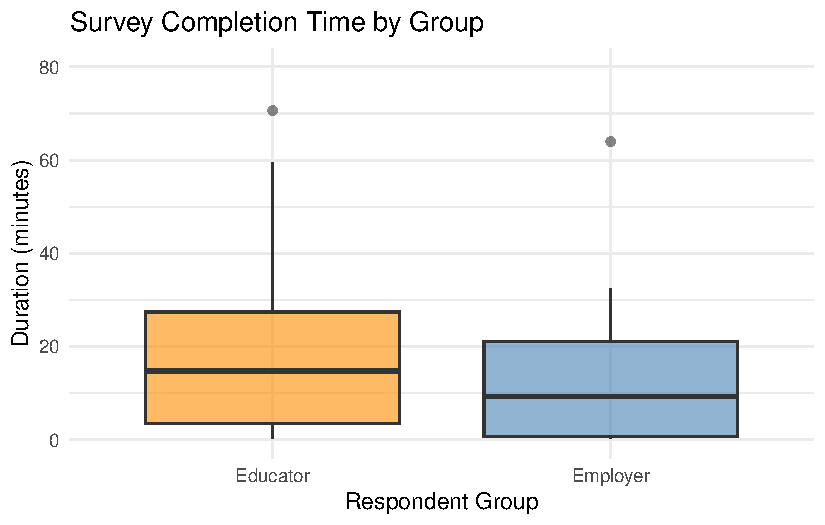
\includegraphics{Final-Project_files/figure-pdf/Data_Desc_01-1.pdf}

}

\caption{Assessing survey elapsed time distribution via box plots to
understand engagement by survey group.}

\end{figure}

Survey completion time differed by group. Educators, on average, spent
more time completing the survey than employers. While no follow-up
question asked participants to explain their response time, this
discrepancy may reflect greater engagement or a tendency for more
elaborated responses among educators. It may also suggest a greater
willingness among educators to participate more thoughtfully. The box
plot below illustrates the distribution of survey duration (in minutes)
by group.

\begin{figure}[H]

{\centering 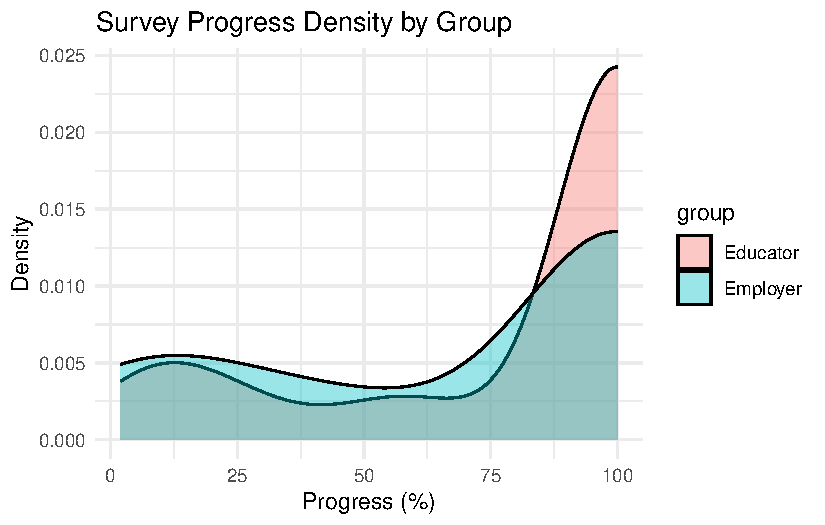
\includegraphics{Final-Project_files/figure-pdf/Data_Desc_02-1.pdf}

}

\caption{Assessing survey completion as a density curve to understand
engagement by survey group.}

\end{figure}

Regarding the proportion of the survey completed, employer responses
were more variable---spanning the full range from partial to full
completion. In contrast, educators tended to complete more of the
survey, with a concentration near full completion and a less pronounced
left tail. The density plot below visualizes these differences in survey
progress across groups.

\begin{figure}[H]

{\centering 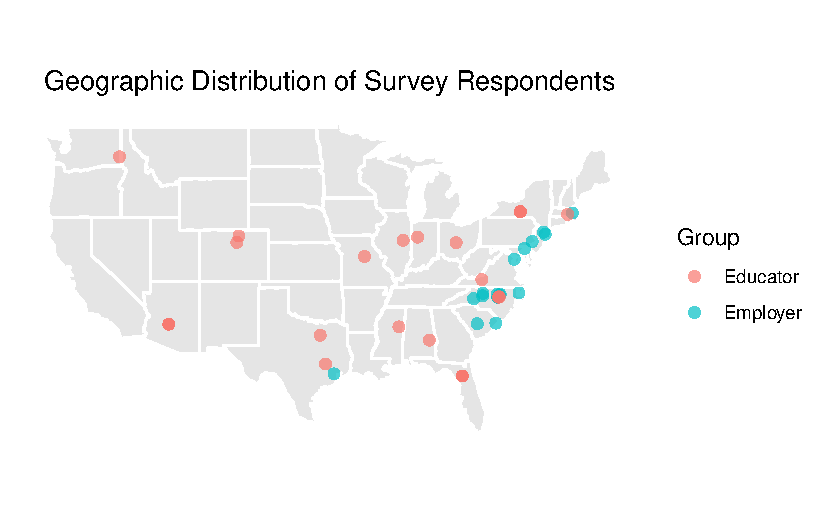
\includegraphics{Final-Project_files/figure-pdf/Data_Desc_06-1.pdf}

}

\caption{Geographic distribution of survey respondents across the United
States.}

\end{figure}

Since our analysis focused on the representativeness of the United
States, we identified three sets of coordinates in the educator dataset
corresponding to international institutions: the University of Guelph in
Ontario, Canada; Zanzibar University in Chake, Tanzania; and Chiba
University in Chiba, Japan. Employer survey participants were
predominantly sampled from locations along the eastern seaboard of the
United States, while educators were more widely distributed across the
country. We highlight this to illustrate that perceptions of veterinary
dental students---particularly among employers---may differ for
individuals located far from the regions where most participants were
sampled. Additionally, because many of the responses came from major
metropolitan areas, our findings may underrepresent opinions regarding
student knowledge gaps in more rural settings.

\hypertarget{educator-metrics}{%
\paragraph{Educator metrics}\label{educator-metrics}}

\begin{figure}[H]

{\centering 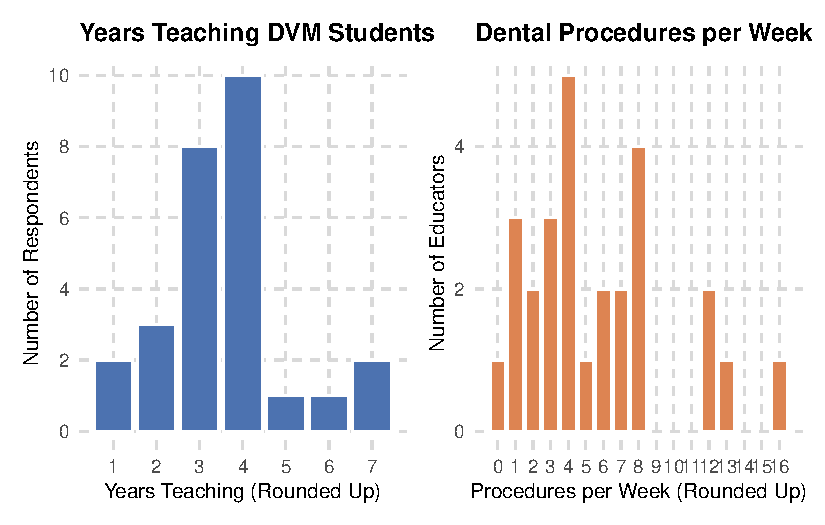
\includegraphics{Final-Project_files/figure-pdf/Data_Desc_03-1.pdf}

}

\caption{Educator contextualized background information about teaching
and procedures.}

\end{figure}

Figure 3.3 provides an overview of the survey participants and their
institutions. Most respondents reported having between 2 and 4 years of
experience teaching veterinary students in clinical training. The
distribution of years taught appears approximately normal, with fewer
educators at the lower and upper ends of the experience range.
Respondents also reported the number of dental procedures performed by
their primary care service each week. While some outliers from busier
institutions reported higher volumes, most educators estimated
performing between 1 and 8 procedures per week.

\hypertarget{employer-metrics}{%
\paragraph{Employer metrics}\label{employer-metrics}}

\begin{longtable}[]{@{}lrr@{}}
\caption{Job Setting or Organization: Counts and
Percentages}\tabularnewline
\toprule\noalign{}
Job Setting & Count & Percentage \\
\midrule\noalign{}
\endfirsthead
\toprule\noalign{}
Job Setting & Count & Percentage \\
\midrule\noalign{}
\endhead
\bottomrule\noalign{}
\endlastfoot
Group corporate veterinary practice & 2 & 16.7 \\
Independently owned group veterinary practice & 2 & 16.7 \\
Independently owned single veterinary practice & 7 & 58.3 \\
Industry/commercial & 1 & 8.3 \\
\end{longtable}

\begin{longtable}[]{@{}lrr@{}}
\caption{Respondent Role: Counts and Percentages}\tabularnewline
\toprule\noalign{}
Respondent Role & Count & Percentage \\
\midrule\noalign{}
\endfirsthead
\toprule\noalign{}
Respondent Role & Count & Percentage \\
\midrule\noalign{}
\endhead
\bottomrule\noalign{}
\endlastfoot
Associate veterinarian & 2 & 18.2 \\
Practice manager/HR representative & 2 & 18.2 \\
Practice owner & 7 & 63.6 \\
\end{longtable}

Table 1 and Table 2 provide additional context about the survey
respondents. The majority of respondents work in privately owned
veterinary practices, and most identified themselves as the owners of
those practices.

\begin{figure}[H]

{\centering 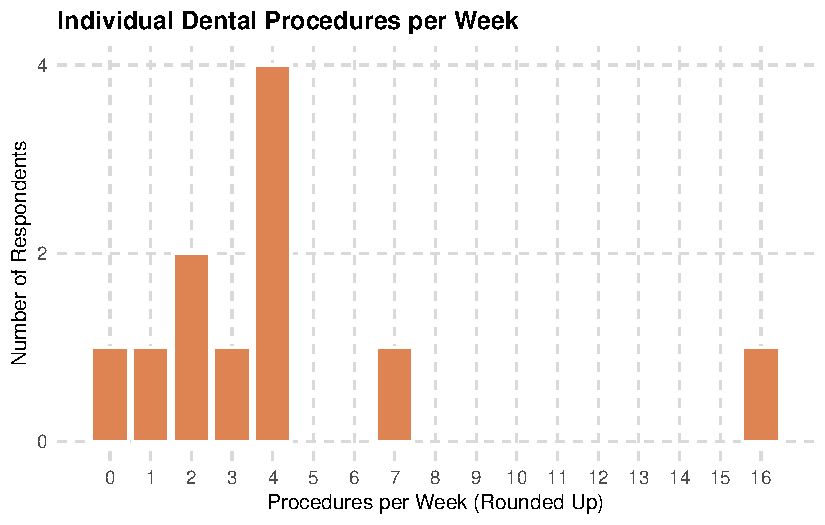
\includegraphics{Final-Project_files/figure-pdf/Data_Desc_05-1.pdf}

}

\caption{Average dental procedures employer survey participants
indicated they performed each week.}

\end{figure}

Figure 3.5 shows that procedure counts tend to be lower in the employer
group compared to the educator group, although the overall distribution
shapes are similar. In both groups, the data exhibit a right-skewed
pattern, with most respondents reporting lower procedure counts and a
few outliers representing higher volumes. This pattern aligns with the
intuitive understanding that while some practices or institutions have
greater clinical demands on veterinarians, these cases are less
common---at least based on the survey responses.

\hypertarget{data-source}{%
\subsection{Data Source}\label{data-source}}

Survey data were collected using Qualtrics, a cloud-based experience
management platform commonly used for gathering feedback and sentiment
across workforce domains. Participants from the educator survey were
recruited via email invitation sent by the researcher, using
pre-existing contact lists. Dr.~Ross-Estrada distributed the employer
survey to her personal and professional networks online. Participation
was voluntary and anonymous. There was no incentive offered for
completing the survey.

\hypertarget{preprocessing-description}{%
\subsection{Preprocessing Description}\label{preprocessing-description}}

Although the employer and educator data sets shared a similar structure,
they were not identical. Most pre-processing steps were applied
uniformly across both data sets, with minor deviations where needed.

The data sets were imported into the RStudio environment (version
2024.04.1 Build 748). A new variable was created to label the data
source (``Educator'' or ``Employer'') for later grouping and
visualization. The existing respondent\_id column served as a unique
identifier and was treated as the primary key.

Initial cleaning involved removing extraneous metadata included by
Qualtrics---such as survey start and end times, IP addresses,
geolocation data, and question display logic---all of which were
irrelevant to the analysis. These columns were trimmed to streamline the
dataset for subsequent transformation and statistical work.

Column names in the original Qualtrics export were alphanumeric but
often ambiguous and misleading. Many variable names did not match the
corresponding survey question numbers. Our team manually mapped the
exported column names to their corresponding survey questions and
responses by referencing adjacent metadata fields and using deductive
reasoning. This process allowed us to build an index-based column naming
structure, which greatly improved the manageability and interpretability
of the dataset.

Before diving into question-specific analysis, we first identified the
subset of survey questions relevant to our research objectives. All
unrelated or out-of-scope items were removed. This step reduced the
employer dataset from 176 columns to 100, and the educator dataset from
171 columns to 102.

Several formatting inconsistencies also needed to be resolved. Some
multi-select questions appeared in the form of comma-separated text
responses within a single column, while others were exported into
multiple binary columns. Additionally, for certain questions, a response
option that received zero selections was dropped entirely by Qualtrics.
To standardize these issues, we implemented a script to ``explode''
comma-separated responses into individual binary columns. For dropped
columns, we manually reintroduced them as zero-filled dummy variables to
preserve the full response structure.

Finally, we filtered out participants who answered less than half of the
survey. We also excluded:

\begin{itemize}
\item
  Employers who responded ``No'' to the question: ``Do you work with
  early career veterinarians (someone who has graduated from a DVM
  program after May 2021)?''
\item
  Educators who responded ``No'' to: ``Do you teach in any capacity of
  the dental curriculum at your institution?''
\end{itemize}

After all preprocessing steps, the final cleaned datasets consisted of
13 employer participants and 30 educator participants.

\hypertarget{statistical-methods}{%
\section{Statistical Methods}\label{statistical-methods}}

\hypertarget{method-description}{%
\subsection{Method Description}\label{method-description}}

Likert scale questions (statistical questions \#1,3, 6, and 8): These
questions utilize a likert scale to answer Strongly Agree, Agree,
Disagree, or Strongly Disagree on a variety of skills and procedures. To
analyze this data, we will use diverging stacked bar charts and tables
for exploratory data analysis and the Mann-Whitney U Test for the formal
hypothesis procedure. The Mann-Whitney U Test is a non-parametric test
that does not rely on an assumption of normality. It does require
independence between datasets and it is reasonable to assume that the
educators and employers were independent from each other when taking the
survey. The Mann-Whitney test particularly works well with these
questions due to the ordinal (and therefore ranked) nature of the data.

Select all that apply questions (statistical questions \#2, 5, and 7):
These questions asked the participants to ``select all that apply'' as
it relates to skills in pre-clinical curriculum, format of dental
instruction, and skills for clinical training respectively. We will
utilize frequency tables and bar plots to explore the data for these
questions and use Fisher's Exact Test as a formal inference procedure
for the comparison of the two groups. Fisher's Exact Test works with
categorical data with independent samples, in this case educators and
employers. In this context, it is preferred over Chi-Squared Tests due
to the small sample size and therefore not meeting the expected count
threshold that is required to proceed with Chi-Squared Tests. Given the
small sample sizes, we acknowledge the limited power of these analyses
and may consider post hoc power analyses for these tests.

Numerical entry questions: (statistical question \#4): This question
asks participants to enter a number related to the number of dental
procedures that should be completed during training in different areas.
We plan to produce box plots and/or histograms to visually examine the
data. Depending on the normality or lack thereof of the distributions,
we will then conduct either a two-sample t-test or a Mann-Whitney U
Test. As mentioned above, the Mann Whitney U test is a non-parametric
test that does not depend on the assumption of normality. If the
assumption on normality is met, we can consider a two-sample t test for
this analysis.

\hypertarget{results}{%
\section{Results}\label{results}}

\hypertarget{s1-are-there-significant-differences-between-educators-and-practice-owners-in-their-belief-that-new-graduates-are-competent-in-key-dental-skills-on-their-first-day-of-practice}{%
\subsubsection{S1 Are there significant differences between educators
and practice owners in their belief that new graduates are competent in
key dental skills on their first day of
practice?}\label{s1-are-there-significant-differences-between-educators-and-practice-owners-in-their-belief-that-new-graduates-are-competent-in-key-dental-skills-on-their-first-day-of-practice}}

\hypertarget{s2-is-there-a-difference-between-educators-and-practice-owners-in-their-reports-educators-actual-teaching-vs.-owners-perceptions-of-which-dental-skills-were-taught-in-the-pre-clinical-dvm-curriculum-for-recent-graduates}{%
\subsubsection{S2 Is there a difference between educators and practice
owners in their reports (educators' actual teaching vs.~owners'
perceptions) of which dental skills were taught in the pre-clinical DVM
curriculum for recent
graduates?}\label{s2-is-there-a-difference-between-educators-and-practice-owners-in-their-reports-educators-actual-teaching-vs.-owners-perceptions-of-which-dental-skills-were-taught-in-the-pre-clinical-dvm-curriculum-for-recent-graduates}}

\hypertarget{s3-is-there-a-difference-between-educators-and-practice-owners-in-their-level-of-agreement-about-whether-specific-dental-skills-should-be-taught-pre-clinically}{%
\subsubsection{S3 Is there a difference between educators and practice
owners in their level of agreement about whether specific dental skills
should be taught
pre-clinically?}\label{s3-is-there-a-difference-between-educators-and-practice-owners-in-their-level-of-agreement-about-whether-specific-dental-skills-should-be-taught-pre-clinically}}

\hypertarget{s4-do-employers-and-educators-differ-in-their-expectations-about-how-many-dental-procedures-new-graduates-should-complete-during-clinical-training}{%
\subsubsection{S4 Do employers and educators differ in their
expectations about how many dental procedures new graduates should
complete during clinical
training?}\label{s4-do-employers-and-educators-differ-in-their-expectations-about-how-many-dental-procedures-new-graduates-should-complete-during-clinical-training}}

\hypertarget{s5-is-there-difference-between-the-instructional-formats-in-dentistry-reported-by-dvm-programs-and-the-formats-perceived-by-employers-to-have-been-completed-by-early-career-veterinarians}{%
\subsubsection{S5 Is there difference between the instructional formats
in dentistry reported by DVM programs and the formats perceived by
employers to have been completed by early career
veterinarians?}\label{s5-is-there-difference-between-the-instructional-formats-in-dentistry-reported-by-dvm-programs-and-the-formats-perceived-by-employers-to-have-been-completed-by-early-career-veterinarians}}

Both educators and employers were asked a question relating to the
format of instruction during the clinical year.

On question 20 of their survey, employers were asked: ``What format of
clinical instruction in dentistry do you believe that the early career
veterinarians (individuals who have graduated from a DVM program after
May 2021) hired into your practice/organization/institution completed as
part of their DVM training? Select all that apply.''

On question 16 of their survey, educators were asked: ``What format of
instruction in dentistry does your DVM program provide during the
clinical year? Select all that apply.''

Since the question was of the format ``select all that apply,''
participants were able to select more than one response and percentages
will not add to 100\%. Results reported below are the percentages of
their respective group (educators or employers) that selected the given
format of instruction. Percentages were utilized due to the difference
in sample size.

Educators and employers were also given the option to enter their own
responses to the question. One employer opted to write in ``Cadaver.''
Two educators entered their own responses with one saying ``rounds'' and
the other saying ``topic seminars do occur with some rotations during
case rounds when dental cases are chosen to present.''

Educators and employers differed in their perceptions of clinical dental
instruction formats completed by early career veterinarians. While a
majority in both groups acknowledged didactic instruction, educators
reported higher rates of wet lab (73.3\% vs.~46.2\%) and live patient
training (93.3\% vs.~38.5\%) compared to employers. Conversely,
employers more frequently identified simulation training (30.8\%
vs.~16.7\%) than educators. These differences suggest varying
expectations or awareness between the two groups regarding dental
training experiences of recent graduates.

\begin{figure}[H]

{\centering 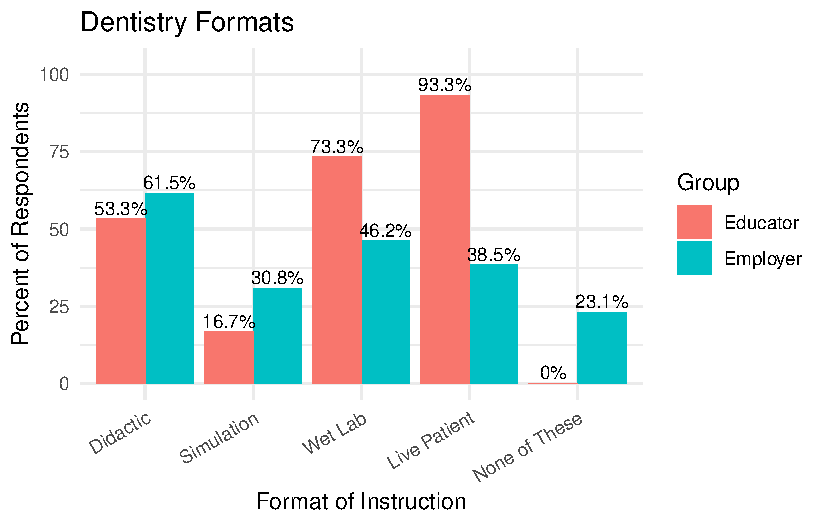
\includegraphics{Final-Project_files/figure-pdf/formatgraph-1.pdf}

}

\caption{Perceived Clinical Instruction Formats in Dentistry Completed
by Early Career Veterinarians}

\end{figure}

Figure 5.1 shows the percentages of each format selected and Table 3
shows the p-value associated with performing Fisher's Exact Test on each
format.

Didactic instruction was selected by 53.3\% of educators and 61.5\% of
employers, with no statistically significant difference between the
groups (p=0.743). There was also no statistically significant difference
in simulation (p=0.417) and wet lab instruction (p=0.162).

On the other hand, live patient instruction was selected by 93.3\% of
educators, but only 38.5\% of employers. This difference was found to be
statistically significant with a p-value of 0.0003.

``None of these'' was also found to be statistically significant at the
5\% level. No educators selected that none of these formats were used,
but 23.1\% of employers selected that none of the formats were believed
to be utilized in the clinical year.

\begin{longtable}[]{@{}
  >{\raggedright\arraybackslash}p{(\columnwidth - 6\tabcolsep) * \real{0.1867}}
  >{\raggedleft\arraybackslash}p{(\columnwidth - 6\tabcolsep) * \real{0.3200}}
  >{\raggedleft\arraybackslash}p{(\columnwidth - 6\tabcolsep) * \real{0.3200}}
  >{\raggedright\arraybackslash}p{(\columnwidth - 6\tabcolsep) * \real{0.1733}}@{}}
\caption{Perceived Formats of Clinical Dental Instruction in DVM
Programs}\tabularnewline
\toprule\noalign{}
\begin{minipage}[b]{\linewidth}\raggedright
Format
\end{minipage} & \begin{minipage}[b]{\linewidth}\raggedleft
\% of Educators Selected
\end{minipage} & \begin{minipage}[b]{\linewidth}\raggedleft
\% of Employers Selected
\end{minipage} & \begin{minipage}[b]{\linewidth}\raggedright
P-value
\end{minipage} \\
\midrule\noalign{}
\endfirsthead
\toprule\noalign{}
\begin{minipage}[b]{\linewidth}\raggedright
Format
\end{minipage} & \begin{minipage}[b]{\linewidth}\raggedleft
\% of Educators Selected
\end{minipage} & \begin{minipage}[b]{\linewidth}\raggedleft
\% of Employers Selected
\end{minipage} & \begin{minipage}[b]{\linewidth}\raggedright
P-value
\end{minipage} \\
\midrule\noalign{}
\endhead
\bottomrule\noalign{}
\endlastfoot
Didactic & 53.3 & 61.5 & 0.743 \\
Simulation & 16.7 & 30.8 & 0.417 \\
Wet Lab & 73.3 & 46.2 & 0.162 \\
Live Patient & 93.3 & 38.5 & 0.000303 *** \\
None of These & 0.0 & 23.1 & 0.0232 * \\
\end{longtable}

\hypertarget{s6-do-educators-and-employers-differ-in-their-views-on-which-formats-of-clinical-instruction-in-dentistry-should-be-required-for-dvm-students-as-part-of-their-clinical-training}{%
\subsubsection{S6 Do educators and employers differ in their views on
which formats of clinical instruction in dentistry should be required
for DVM students as part of their clinical
training?}\label{s6-do-educators-and-employers-differ-in-their-views-on-which-formats-of-clinical-instruction-in-dentistry-should-be-required-for-dvm-students-as-part-of-their-clinical-training}}

In question \#21 of the employers version of the survey, participants
were asked, ``Which of the following types of \ul{\emph{clinical
instruction in dentistry}} do you think that DVM students should be
required to complete as part of a \ul{\emph{DVM program}}? Select one
response for each of the instructional types listed below.'' The
analogue of this question for educators was survey question \#17. We
want to make a note that the educators survey question had a slight
variation in phraseology. It asked, ``Which of the following types of
\ul{\emph{instruction}} do you think DVM students should be required to
complete as part of their \ul{\emph{clinical training}}? Select one
response for each type of instruction listed below.''.

This question is targeting how participants feel about what dental
veterinarian medical programs are teaching and what topics should be
required in their curriculum. The research question asked if there was a
difference in opinions on this matter. To infer from the data, we will
use the Mann-Whitney U-Test, a non-parametric test also known as
Wilcoxin Rank Sign Test. This test assumes mutual exclusivity between
groups.

\begin{verbatim}
       question     W     p_value significance
Q17_01   Q17_01 138.5 0.414724985           ns
Q17_02   Q17_02 108.0 0.362883946           ns
Q17_03   Q17_03 162.0 0.712880664           ns
Q17_04   Q17_04 263.5 0.002740855           **
Q17_05   Q17_05    NA          NA         <NA>
Q17_06   Q17_06    NA          NA         <NA>
Q17_07   Q17_07    NA          NA         <NA>
\end{verbatim}

\hypertarget{s7-is-there-a-difference-between-the-clinical-dentistry-skills-that-educators-report-dvm-students-are-learning-during-their-clinical-training-and-the-skills-that-employers-believe-recent-graduates-have-completed-as-part-of-their-dvm-program}{%
\subsubsection{S7 Is there a difference between the clinical dentistry
skills that educators report DVM students are learning during their
clinical training and the skills that employers believe recent graduates
have completed as part of their DVM
program?}\label{s7-is-there-a-difference-between-the-clinical-dentistry-skills-that-educators-report-dvm-students-are-learning-during-their-clinical-training-and-the-skills-that-employers-believe-recent-graduates-have-completed-as-part-of-their-dvm-program}}

Both educators and employers were asked a question related to skills
learned and practiced during the clinical year.

On question 25 of their survey, employers were asked: ``Which of the
following skills do you think that individuals who graduated with a DVM
degree after May 2021 completed during the clinical training portion of
their DVM program? Select all that apply.''

On question 20 of their survey, educators were asked: ``Which of the
following skills are DVM students at your institution
practicing/learning during the clinical training portion of the DVM
program? Select all that apply.''

Since the question was of the format ``select all that apply,''
participants were able to select more than one response and percentages
will not add to 100\%. Results reported below are the percentages of
their respective group (educators or employers) that selected the given
format of instruction. Percentages were utilized due to the difference
in sample size.

Educators and employers were also given the option to enter their own
responses to the question. No employers entered any text responses. Six
educators entered text responses of the following:

\begin{itemize}
\tightlist
\item
  ``OvaVet gel application, Crown amputation, Sealant application for
  UCF, oral tumor biopsy and excision, orthodontia''
\item
  ``Nerve blocks, barrier sealant and bonded sealant application, jaw
  fracture repair, root canals''
\item
  ``Often- bonded sealants; Sometimes- root canals, restorations, jaw
  fracture repair''
\item
  ``Oral biopsy, root planning, bonded sealants''
\item
  ``extractions only if performed on that patient''
\item
  ``Not all students see all types of extractions''
\end{itemize}

\begin{figure}[H]

{\centering 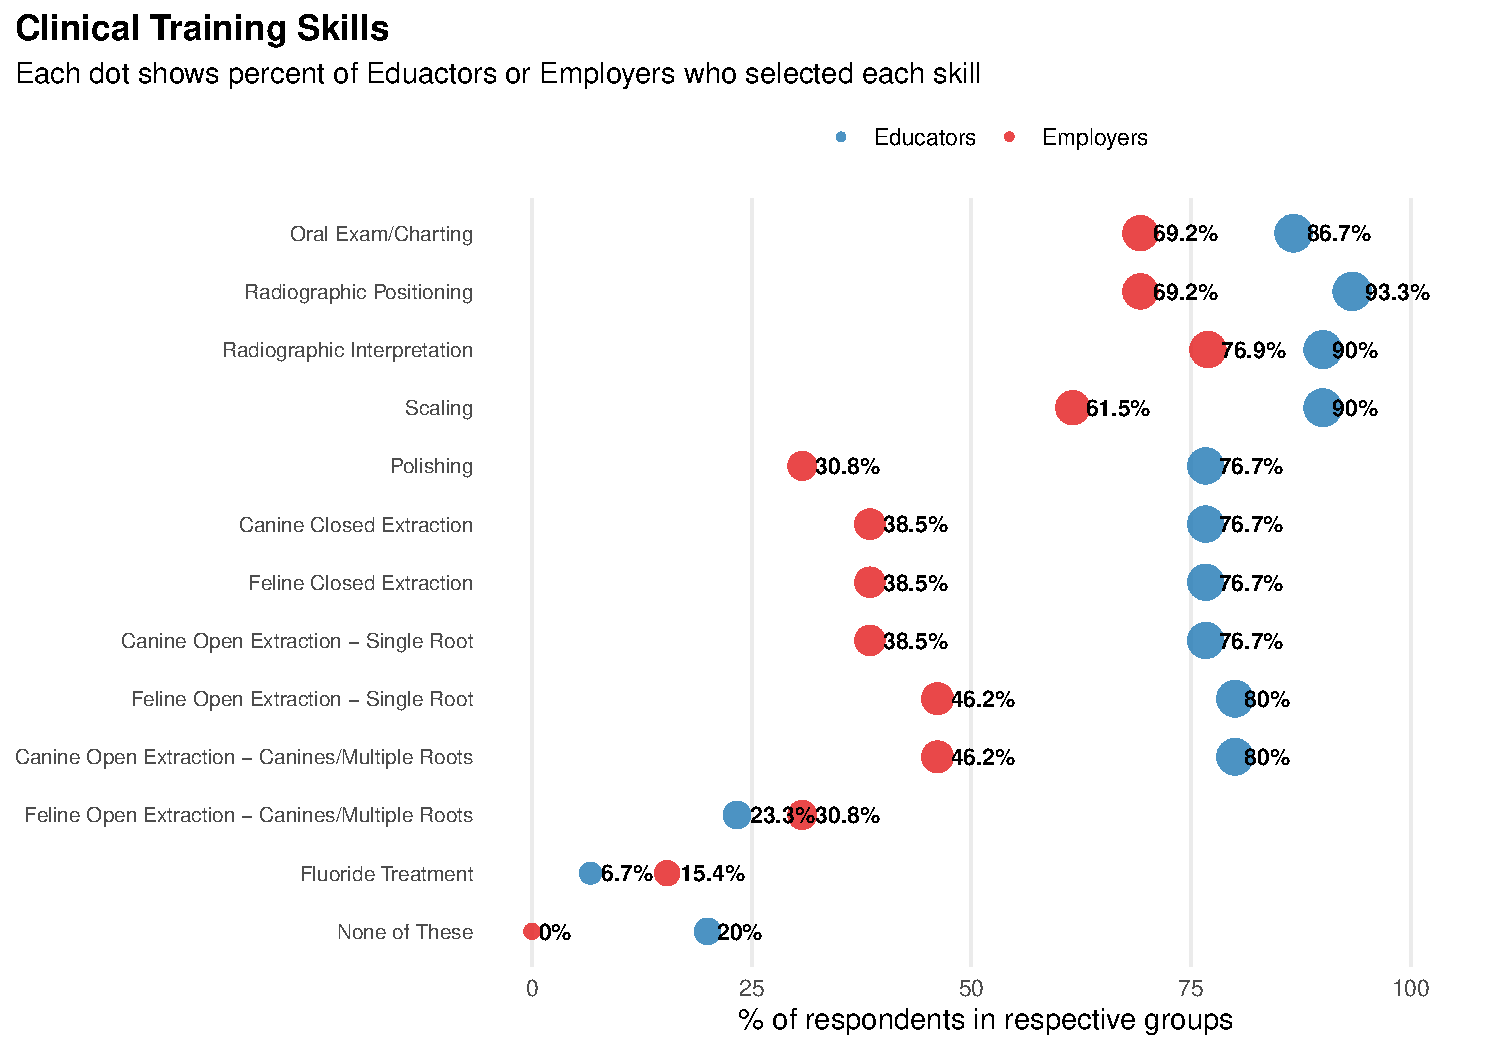
\includegraphics{Final-Project_files/figure-pdf/question_7a-1.pdf}

}

\caption{Clinical Training Skills Perceived by Educators vs Employers in
DVM Programs}

\end{figure}

\begin{longtable}[]{@{}
  >{\raggedright\arraybackslash}p{(\columnwidth - 6\tabcolsep) * \real{0.5581}}
  >{\raggedleft\arraybackslash}p{(\columnwidth - 6\tabcolsep) * \real{0.1744}}
  >{\raggedleft\arraybackslash}p{(\columnwidth - 6\tabcolsep) * \real{0.1744}}
  >{\raggedright\arraybackslash}p{(\columnwidth - 6\tabcolsep) * \real{0.0930}}@{}}
\caption{Perceived Skills Learned of Clinical Dental Instruction in DVM
Programs}\tabularnewline
\toprule\noalign{}
\begin{minipage}[b]{\linewidth}\raggedright
Skill
\end{minipage} & \begin{minipage}[b]{\linewidth}\raggedleft
\% of Educators
\end{minipage} & \begin{minipage}[b]{\linewidth}\raggedleft
\% of Employers
\end{minipage} & \begin{minipage}[b]{\linewidth}\raggedright
P-value
\end{minipage} \\
\midrule\noalign{}
\endfirsthead
\toprule\noalign{}
\begin{minipage}[b]{\linewidth}\raggedright
Skill
\end{minipage} & \begin{minipage}[b]{\linewidth}\raggedleft
\% of Educators
\end{minipage} & \begin{minipage}[b]{\linewidth}\raggedleft
\% of Employers
\end{minipage} & \begin{minipage}[b]{\linewidth}\raggedright
P-value
\end{minipage} \\
\midrule\noalign{}
\endhead
\bottomrule\noalign{}
\endlastfoot
Oral Exam/Charting & 86.7 & 69.2 & 0.21700 \\
Radiographic Positioning & 93.3 & 69.2 & 0.05760 \\
Radiographic Interpretation & 90.0 & 76.9 & 0.34500 \\
Scaling & 90.0 & 61.5 & 0.04150 \\
Polishing & 76.7 & 30.8 & 0.00672 \\
Canine Closed Extraction & 76.7 & 38.5 & 0.03390 \\
Feline Closed Extraction & 76.7 & 38.5 & 0.03390 \\
Canine Open Extraction - Single Root & 76.7 & 38.5 & 0.03390 \\
Feline Open Extraction - Single Root & 80.0 & 46.2 & 0.03670 \\
Canine Open Extraction - Canines/Multiple Roots & 80.0 & 46.2 &
0.03670 \\
Feline Open Extraction - Canines/Multiple Roots & 23.3 & 30.8 &
0.70900 \\
Fluoride Treatment & 6.7 & 15.4 & 0.57200 \\
None of These & 20.0 & 0.0 & 0.15500 \\
\end{longtable}

\hypertarget{s8-do-educators-and-employers-differ-in-their-opinions-about-which-clinical-dentistry-skills-dvm-students-should-be-required-to-practice-or-learn-during-their-clinical-training}{%
\subsubsection{S8 Do educators and employers differ in their opinions
about which clinical dentistry skills DVM students should be required to
practice or learn during their clinical
training?}\label{s8-do-educators-and-employers-differ-in-their-opinions-about-which-clinical-dentistry-skills-dvm-students-should-be-required-to-practice-or-learn-during-their-clinical-training}}

In question \#26 of the employers version of the survey, participants
were asked, ``Which of the following skills do you think that DVM
students should be required to practice/learn as part of the clinical
training portion of a DVM program? Select one response for each of the
skills listed below.'' The analogue of this question for educators was
survey question \#21

This question hits at the sentiment on what both groups think should be
required practice/learnings for students. The research question asked if
there was a difference in opinions on this matter. To infer from the
data, we will use the Mann-Whitney U-Test, a non-parametric test also
known as Wilcoxin Rank Sign Test. This test assumes mutual exclusivity
between groups.

\begin{verbatim}
       question     W    p_value significance
Q21_01   Q21_01 139.0 0.62171592           ns
Q21_02   Q21_02 157.0 0.71723375           ns
Q21_03   Q21_03 126.5 0.19379896           ns
Q21_04   Q21_04 156.0 0.76158684           ns
Q21_05   Q21_05 148.5 1.00000000           ns
Q21_06   Q21_06 127.5 0.32836731           ns
Q21_07   Q21_07 104.5 0.04863265            *
Q21_08   Q21_08 104.5 0.04892603            *
Q21_09   Q21_09 115.5 0.07564530            .
Q21_10   Q21_10 115.5 0.07587786            .
Q21_11   Q21_11  54.0 0.20728866           ns
Q21_12   Q21_12    NA         NA         <NA>
Q21_13   Q21_13    NA         NA         <NA>
Q21_14   Q21_14    NA         NA         <NA>
\end{verbatim}

\begin{Shaded}
\begin{Highlighting}[]
\FunctionTok{view}\NormalTok{(Educator\_Data\_Clean }\SpecialCharTok{\%\textgreater{}\%} \FunctionTok{select}\NormalTok{(}\FunctionTok{starts\_with}\NormalTok{(}\StringTok{"Q17"}\NormalTok{)))}
\FunctionTok{view}\NormalTok{(Employer\_Data\_Clean }\SpecialCharTok{\%\textgreater{}\%} \FunctionTok{select}\NormalTok{(}\FunctionTok{starts\_with}\NormalTok{(}\StringTok{"Q21"}\NormalTok{)))}
\end{Highlighting}
\end{Shaded}

\hypertarget{findings}{%
\subsection{Findings}\label{findings}}

\hypertarget{statistical-analysis}{%
\subsection{Statistical Analysis}\label{statistical-analysis}}

\hypertarget{discussionconclusion}{%
\section{Discussion/Conclusion}\label{discussionconclusion}}

\hypertarget{interpretation-of-results}{%
\subsection{Interpretation of Results}\label{interpretation-of-results}}

\hypertarget{implications-of-the-study}{%
\subsection{Implications of the Study}\label{implications-of-the-study}}

\hypertarget{limitations}{%
\subsection{Limitations}\label{limitations}}

\hypertarget{recommendations}{%
\subsection{Recommendations}\label{recommendations}}

\hypertarget{summary-of-key-findings}{%
\subsection{Summary of Key Findings}\label{summary-of-key-findings}}

\hypertarget{final-thoughts}{%
\subsection{Final Thoughts}\label{final-thoughts}}

\hypertarget{appendix}{%
\section{Appendix}\label{appendix}}



\end{document}
